\section{Introduction}\label{sec:intro}

A team of language-model agents that packs a bag with two robot arms can fail for at least three different reasons.
A computer-vision Eye may misjudge what is on the table, a planner may order the packing wrongly, or an arm may drop or crush an item.
When the only recorded outcome is \emph{the bag is wrong}, these causes are indistinguishable, and so is the training signal that follows: a reward for the whole team cannot say which agent to improve.
Prior work on language-model robot teams shows that dialogue and modular agents can coordinate arms and embodied agents \citep{mandi2024roco,zhang2024coela}, and a recent benchmark and reinforcement-learning recipe for vision-language embodied cooperation \citep{kang2025vikir} makes the multi-agent setting measurable.
What these systems leave open is attribution: where in the team a failure entered, and how to turn that answer into training data.

\Cref{fig:mechanism} shows the problem on one recorded episode.
The Eye reports the pencil case as \mechPcEye{}\,kg when it weighs \mechPcTrue{}\,kg (\mechPcErr\%) and the notebook as \mechNbEye{}\,kg when it weighs \mechNbTrue{}\,kg (\mechNbErr\%).
The Brain, reasoning correctly from those numbers, stacks the heavier notebook on the lighter pencil case; the team breaks the rule that heavy items go at the bottom and scores \mechNoFixScore{}.
The error is the Eye's, but the failure surfaces in the plan and is only visible in the final bag.
Two mechanisms repair it: an Arm that weighs the item in its gripper can challenge the Eye, and the Arms can weigh every item before planning.
Both are cheap to state and easy to test in a symbolic world, which is why we build the team around interfaces where such evidence can be exchanged.

\begin{figure*}[tbp]
\centering
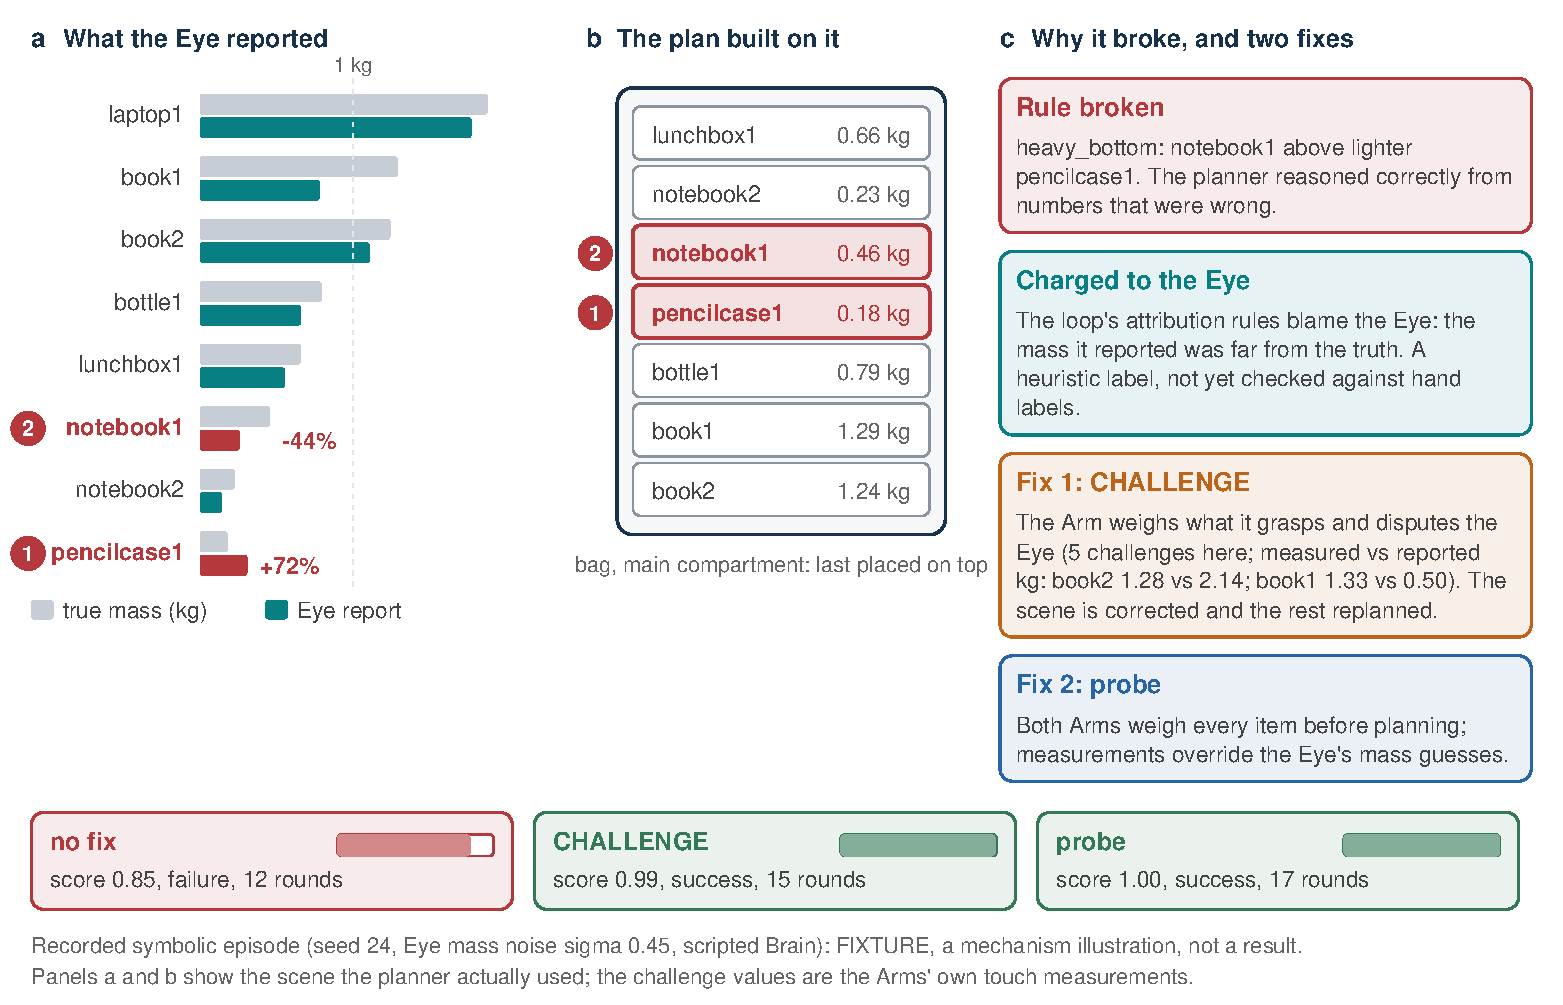
\includegraphics[width=\textwidth]{fig_mechanism}
\caption{\textbf{The problem and our approach (schematic).} (1)~A team of Eyes, a Brain and Arms packs items. Here a heavier item ends up on a lighter one and only one team reward is observed, so it is unclear which agent should learn; typed messages (SCENE, PLAN) make each agent's claims checkable. (2)~We replay the failed episode once per agent, with that agent's contribution replaced by an oracle and all random draws shared; the agent whose replacement repairs the episode carries the responsibility. (3)~Responsibility routes learning: the Eye is updated by credit-guided rejection sampling, the Brain receives the failed episode back as a relabeled, replay-checked example, and an agent that was not to blame is left unchanged. The Eye replay is measured on a recorded fixture episode (seed \mechSeed{}); the Brain and Arm oracle replays drawn here are what the design predicts for that failure and are not yet implemented. Icons are pictograms, not rendered images.}
\label{fig:mechanism}
\end{figure*}

We design the team so that this tracing is possible by construction (\cref{fig:overview}).
\emph{Roles are separated by interface}: only the Eyes receive pixels, only the Brain plans, and the Arms are blind executors that report force and touch.
All communication is a typed, budgeted message (\cref{sec:bus}), so every claim an agent makes about the scene can be compared with what another agent later observes.
The Brain works from a small file-based harness and can check a plan with a deterministic dry run before anything moves (\cref{sec:harness,sec:tools}).
Because the roles are separate, two training signals become natural: replaying an episode with one Eye's report replaced estimates how much that Eye cost the team, and finished episodes, including failed ones, can be relabeled with what the team actually achieved (\cref{sec:signals}).
A single success checker scores the symbolic world and a pose-level simulator and is designed to extend to Isaac Lab (\cref{sec:bridge}), so that a claim made in the cheap world can eventually be re-tested under physics \todo{only the Newton rgb/depth stepping gate G-3 is measured; the manipulation scene and its checker do not exist}.

\paragraph{Contributions.}
\begin{enumerate}[leftmargin=*,itemsep=1pt]
\item A role-separated team design with typed messages, a harness and verification tools in which each failure has an interface to blame (\cref{sec:method}).
\item Two learning signals, counterfactual Eye credit under common random numbers and team hindsight relabeling with a replay check, specified with their assumptions (\cref{sec:signals}).
\item One success definition shared by a symbolic world and a pose-level simulator, designed to extend to Isaac Lab, so plan validity and physical success can be compared \todo{only the gate is measured; no Isaac Lab manipulation result} (\cref{sec:bridge}).
\item An audit of the upstream VIKI-Bench level-2 scorer with a synthetic demonstration, and an evaluation protocol that separates evidence classes (\cref{sec:experiments}).
\end{enumerate}

\paragraph{Status of the evidence.}
This version contains no reportable task-success, benchmark or comparison result.
The system is implemented and its wiring is tested. Gates G-1, G-2, G-3 and G-14 record \emph{engineering} measurements on the real stack --- the Qwen3.5 module map, the DeltaNet fast path, Newton-only rgb/depth stepping on both an RTX 4050 and a Kaggle T4 (a falling cube, stepped on one of the two available devices at a time), and a four-step QLoRA run that resumes mid-epoch from a checkpoint fetched from our private repository; the last is a smoke test, not a trained model. Gate G-6 adds a \emph{simulation-only} impedance cross-check (analytic step error 0.27\,\%, with a push and return measured), not a safety certification. These gates establish that the pipeline runs; they are not evidence about packing performance.
The mechanism figures and appendix~F come from a symbolic fixture with a scripted Brain and parametric Eyes (evidence class FIXTURE), which checks that mechanisms work and says nothing about trained agents.
\todo{Pending, with no report: SimReady asset ingestion and an asset-based kitchen scene; frontier-model CoT (\texttt{RTP\_SERVE\_URL} unset, scripted teacher traces only); training on environment episodes; a fixed held-out test set; omni-model scores; and impedance control on hardware. G-14 is a smoke, not a model-quality result.}
Every unfilled number is a red flag and a row in a machine-readable pending list; \cref{tab:evidence} states the status of each evidence class.
